\documentclass[captions=tableheading]{scrartcl}
\usepackage[aux]{rerunfilecheck}

\usepackage{fontspec}
\usepackage[main=ngerman]{babel}
\usepackage[unicode]{hyperref}
\usepackage{bookmark}
\usepackage{booktabs}
\usepackage{amsmath}
\usepackage{amssymb}
\usepackage{mathtools}
\usepackage{pdfpages}
\setmainfont{Libertinus Serif}
\subject{Versuchsnummer: 303}
\title{Der Lock-In-Verstärker}
\author{Richard Leven \\ \href{mailto:richard.leven@tu-dortmund.de}{richard.leven@tu-dortmund.de}
 \and Joell - D. Jones \\ \href{mailto:joell.jones@tu-dortmund.de}{joell.jones@tu-dortmund.de}} 
\date{
    Durchführung: 19.11.2019\\
    Abgabe: 26.11.2019
}
\publishers{TU Dortmund - Fachschaft Physik}
\begin{document}
\maketitle
\newpage
\section{Ziel}
Kennenlernen des Lock-In-Verstärkers
\section{Theorie}
Ein Lock-In-Verstärker liefert eine klare Gleichspannung bei einem Input von einem Signal mit Rauschen und einem Referenzsignal.
Zuerst werden die zu hohen und zu niedrigen Frequenzen des rauschenden Nutzsignals mit einem Bandpassfilter eliminiert.
Ein Referenzsignal mit gleicher Phase und Frequenz wird nun mit dem Nutzsignal vermischt.
Das resultierende Signal wird mit einem Tiefpassfilter integriert, sodass eine Gleichspannung erzeugt wird, die rauschfrei ist.
\section{Aufgaben}
    \begin{itemize}
        \item{Aufgabe 1 \\}
        Kennenlernen des Schaltkreises des Lock-In-Verstärkers und Ermittlung des konstanten Spannungs-Outputs und variablen Spannungs-Outputs.
        \item{Aufgabe 2 \\}
        Ausgangssignal für 5 verschiedene Phasen messen, mit ausgeschaltetem Noise-Generator.
        \item{Aufgabe 3 \\}
        Wie Aufgabe 2, nur mit Noise-Generator.
        \item{Aufgabe 4 \\}
        Nachweisen eines maximalen Abstandes \(r_{max}\) , in der die Photodiode das Licht einer LED noch messen kann.
        Aufstellen einer Funktion, die die Intensität in Abhängigkeit von \(r\) zeigt.
    \end{itemize}
\section{Versuchsaufbau}

\begin{figure}
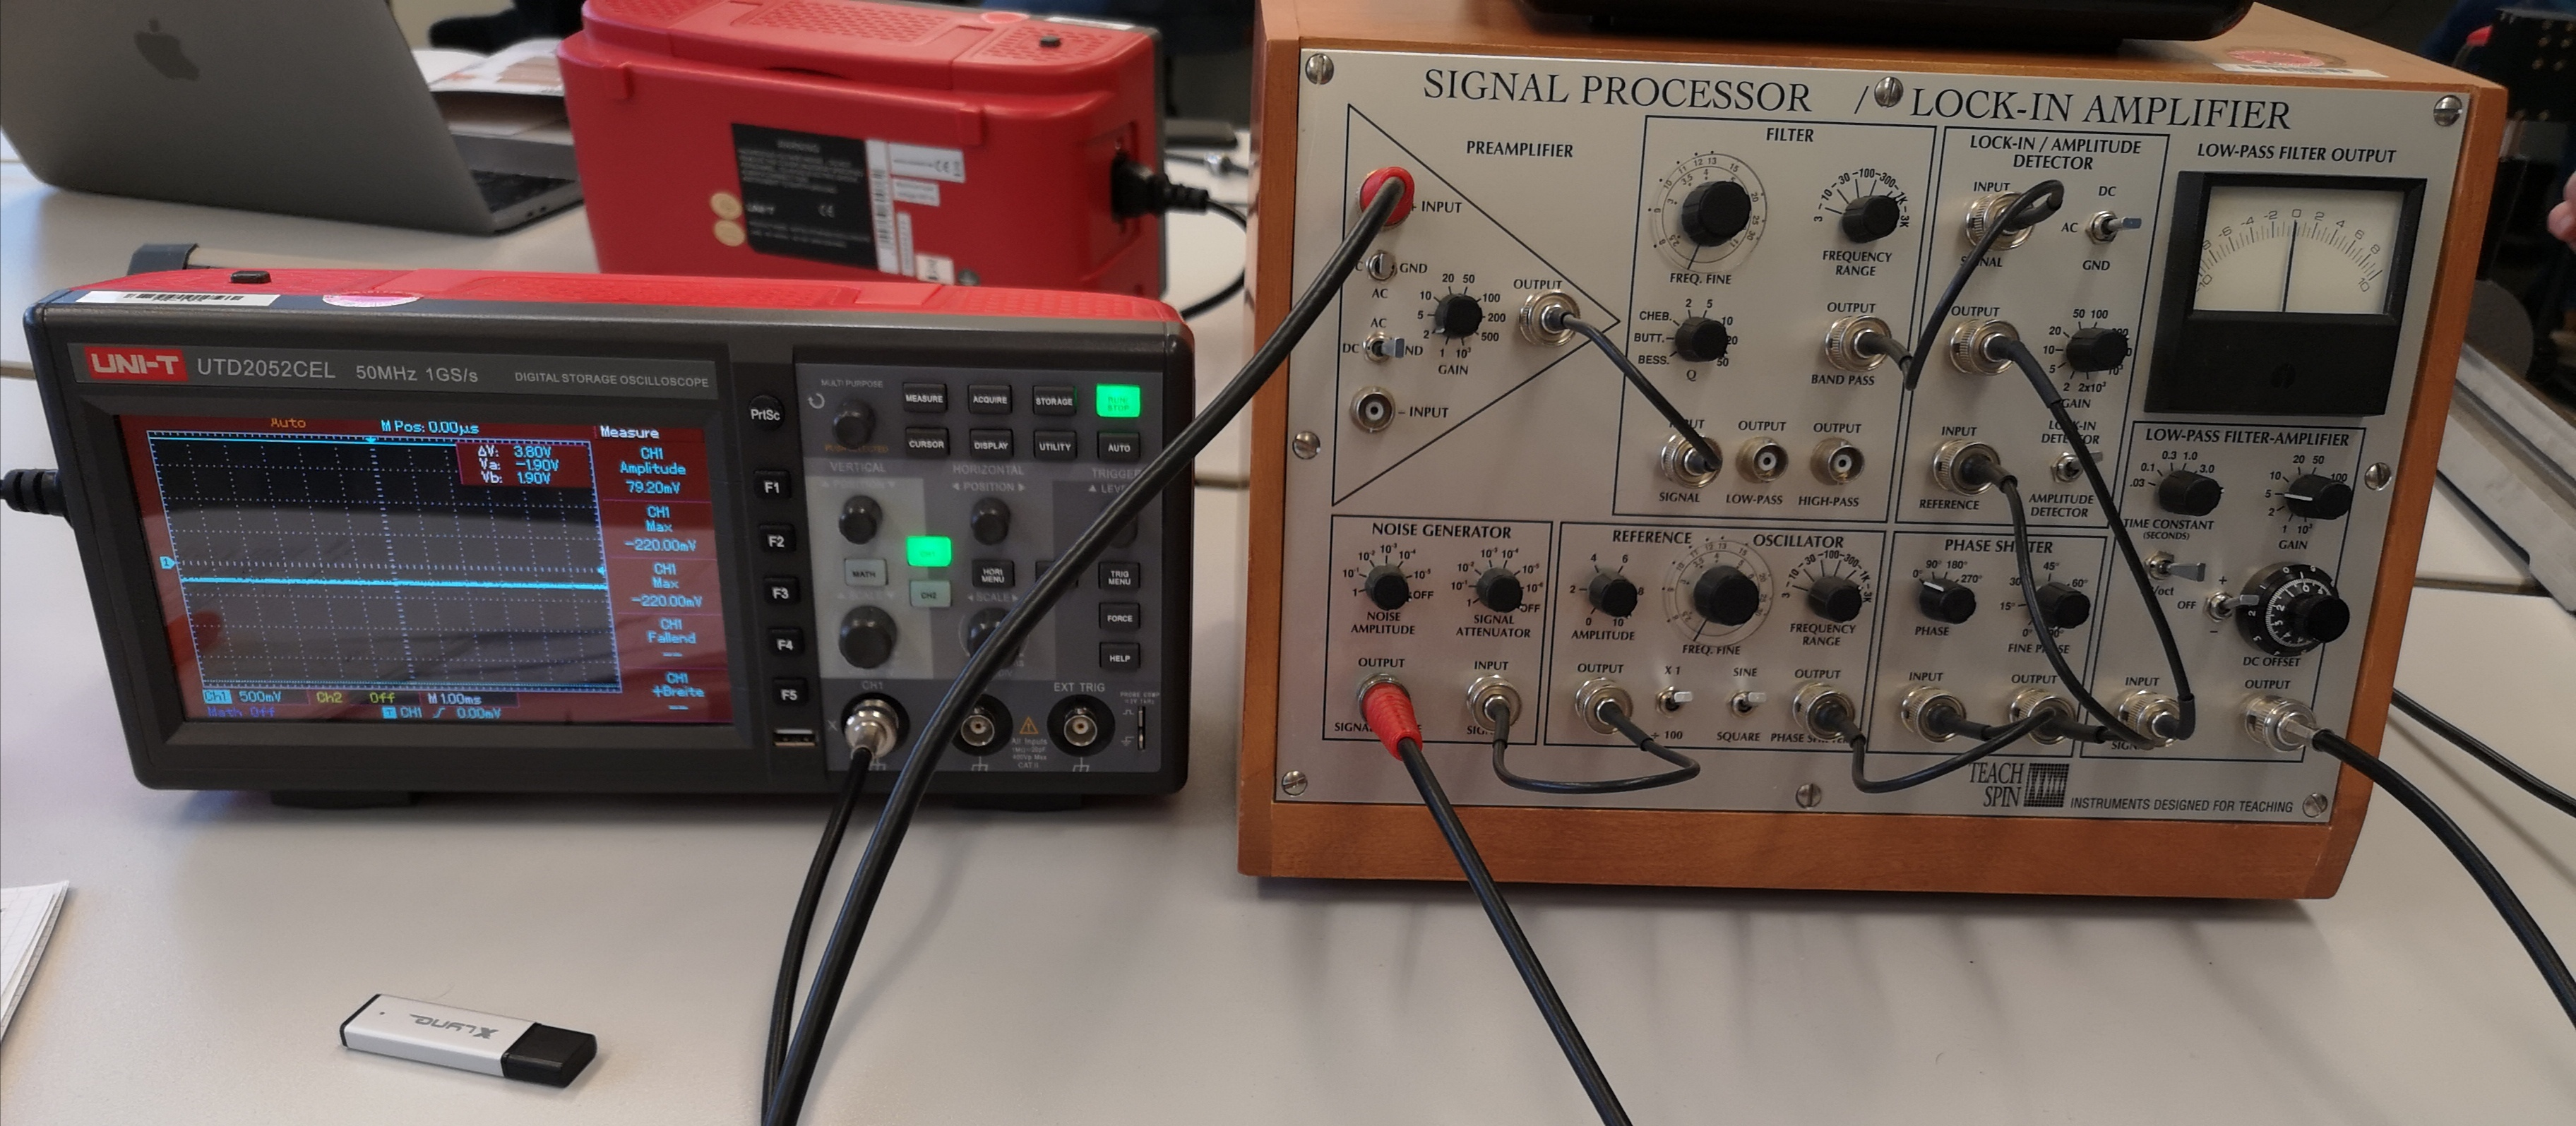
\includepdf[scale=0.5, offset= 0mm -85mm]{Lock_In Bilder/Versauf.jpg}
\end{figure}
\newpage
\section{Versuchsdurchführung}
In Aufgabe 1 wurden die Outputs am Lock-In-Verstärker variiert, sodass einmal der Tiefpass überbrückt wurde und einmal nicht.
Die Outputs wurden an das Oszilloskop angeschlossen und an den Bildschirm angepasst, um ein klares Bild zu bekommen.
\\ \\
In Aufgabe 2 wurde der Tiefpass erneut überbrückt und fünf verschiedene Phaseneinstellungen eingestellt: \(0°, 45°, 90°, 135°, 180°\) \\
Die resultierenden Signale sind in der Auswertung zu sehen.
\\ \\
In Aufgabe 3 wurde das Rauschen auf $10^{-3}$ eingestellt, was der Größenordnung der Spannung des Signals entsprach.
Es wurden danach die gleichen Phasen, wie bei Aufgabe 2 eingestellt.
Die resultierenden Signale sind in der Auswertung zu sehen.
\\ \\
In Aufgabe 4 wurde der Schaltkreis leicht modifiziert, sodass nun der Output vom Lock-In-Verstärker nicht mehr nach dem Tiefpass erfolgte, 
sondern bereits nach dem Lock-In. 
Gleichzeitig wurde auch ein Signal zum Tiefpass-Input gelegt, sodass der Versuchsaufbau nun wie die Schaltkreis-Skizze der Aufgabe 4 geschaltet war.
Die LED wurde mit einer Frequenz von 300Hz betrieben. 
Für eine genauere Messung wurde der Raum verdunkelt und teilweise wurde das Experiment mit Objekten zugedeckt.

\section{Auswertung}

\end{document}